\chapter{Speedy Blinkenlight}
By changing just one line of code, you can control the speed at which the LED on your Arduino blinks.

\GOALS
This chapter introduces how we can give additional information to a procedure to control its behavior. 

\CODE

\lstinputlisting[caption=The {\code blink} procedure is quite handy.,label=code:blink]{code/blink.occ}

% I'm starting to wonder if this is ``Discussion'', or something.. 
\PATTERNS
In the previous chapter, we saw the {\code heartbeat} procedure. In this chapter, we changed line 2. In our first program, we used the \plumbing procedure called {\code heartbeat} to blink the LED. In this chapter, we instead are using {\code blink}, which lets us control both which LED we are blinking as well as the speed at which the LED blinks.

\begin{figure}[h]
  \begin{center}
    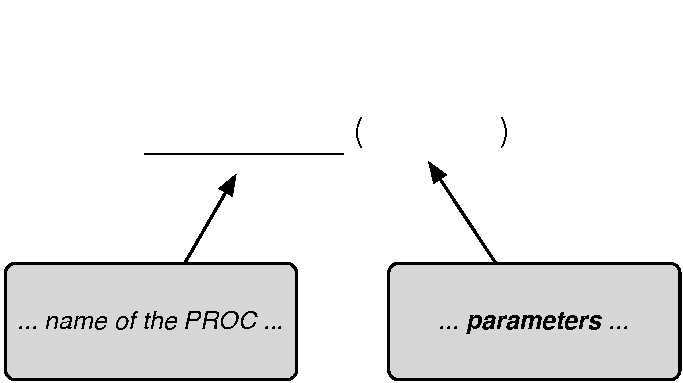
\includegraphics[width=\linewidth]{images/parameter-pattern}
    \caption{Parameters go inside the parentheses of a procedure call.}
    \label{pattern:parameters}
  \end{center}
\end{figure}

On line 2, we can see that a \PROCedure called {\code blink} is being called. This is just like {\code heartbeat}---the code for that procedure is provided by the \plumbing environment. However, instead of an empty set of parentheses, there is stuff in-between them. 

\begin{verbatim}
	blink (13, 500)
\end{verbatim}

These are called {\em parameters}. Parameters are values that we give to procedures that let them do different things based on the values we provide. For example, the first parameter to the procedure {\code blink} is the number {\code 13}. This tells the Arduino which bin it should be turning on and off. Technically, we would say that the pin to which the LED is attached is being driven \HIGH and \LOW. As we explore more of the basics of electronics, you'll come to understand why we say \HIGH and \LOW instead of ``on'' and ``off.''

The second parameter is the amount of time that we want to go by between when the LED is turned on and off. You might think that {\code 500} is a rather large amount of time---until you realize that it is a value in {\em milliseconds}. The prefix {\em milli} means {\em one thousandth}. Therefore, 1000 milliseconds (or 1000ms) equals 1 second. Therefore, half of a second is 500ms, and a tenth of a second is 100ms. 

Parameters are always separated by a comma.

\section{Adding an LED}
You now have enough \plumbing code to add an LED to your Arduino, and control it {\em instead} of the LED on the board!

% XXX Replace me with a hand-drawn picture?
\begin{figure}[h]
  \begin{center}
    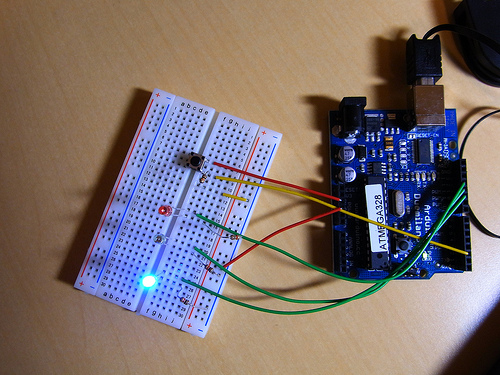
\includegraphics[width=\linewidth]{images/one-led}
    \caption{Connect up one LED to your Arduino.}
    \label{circuit:one-led}
  \end{center}
\end{figure}

Your Arduino will live at the center of a number of increasingly complex circuits. We call them {\em circuits} because they are a circular connection---a loop---that goes through one or more electronic components. In this 